\documentclass{article}

\usepackage{listings}
\usepackage{graphicx}
\usepackage{float}
\usepackage{amsmath}

\author{David Kolden, davidko}
\title{Mandatory assignment 1: Traveling Salesman Problem}

\begin{document}

\maketitle
\tableofcontents

\section{Introduction}
Brief explanation of the assignment, how to start the programs
\section{Exhaustive search}

Start the program with
\begin{lstlisting}[language=bash]
	$ python3 exhaustive.py european_cities.csv 
\end{lstlisting}
The program will find the shortest tour between 6 - 10 cities. The program outputs

\begin{lstlisting}[language=bash]
For n_cities = 6:
Best distance: 5018.8099999999995
Best sequence: (0, 1, 4, 5, 2, 3)
Best order of travel: Barcelona Belgrade Bucharest Budapest Berlin 
Brussels Barcelona
 
For n_cities = 7:
Best distance: 5487.889999999999
Best sequence: (2, 6, 3, 0, 1, 4, 5)
Best order of travel: Berlin Copenhagen Brussels Barcelona Belgrade 
Bucharest Budapest Berlin
 
For n_cities = 8:
Best distance: 6667.489999999999
Best sequence: (3, 7, 0, 1, 4, 5, 2, 6)
Best order of travel: Brussels Dublin Barcelona Belgrade Bucharest 
Budapest Berlin Copenhagen Brussels
 
For n_cities = 9:
Best distance: 6678.549999999999
Best sequence: (2, 6, 8, 3, 7, 0, 1, 4, 5)
Best order of travel: Berlin Copenhagen Hamburg Brussels Dublin 
Barcelona Belgrade Bucharest Budapest Berlin
 
For n_cities = 10:
Best distance: 7486.309999999999
Best sequence: (6, 8, 3, 7, 0, 1, 9, 4, 5, 2)
Best order of travel: Copenhagen Hamburg Brussels Dublin Barcelona 
Belgrade Istanbul Bucharest Budapest Berlin Copenhagen
	 
Time spent[seconds]: [0.002037, 0.015967, 0.134317, 1.310069, 
13.964733]
\end{lstlisting}

The time used by the algorithm to find the best distance was measured. The time spent on solving TSP for six, seven, eight, nine and ten cities is shown in the last two lines of the program output and in figure 1.

\begin{figure}[H]
\begin{center}
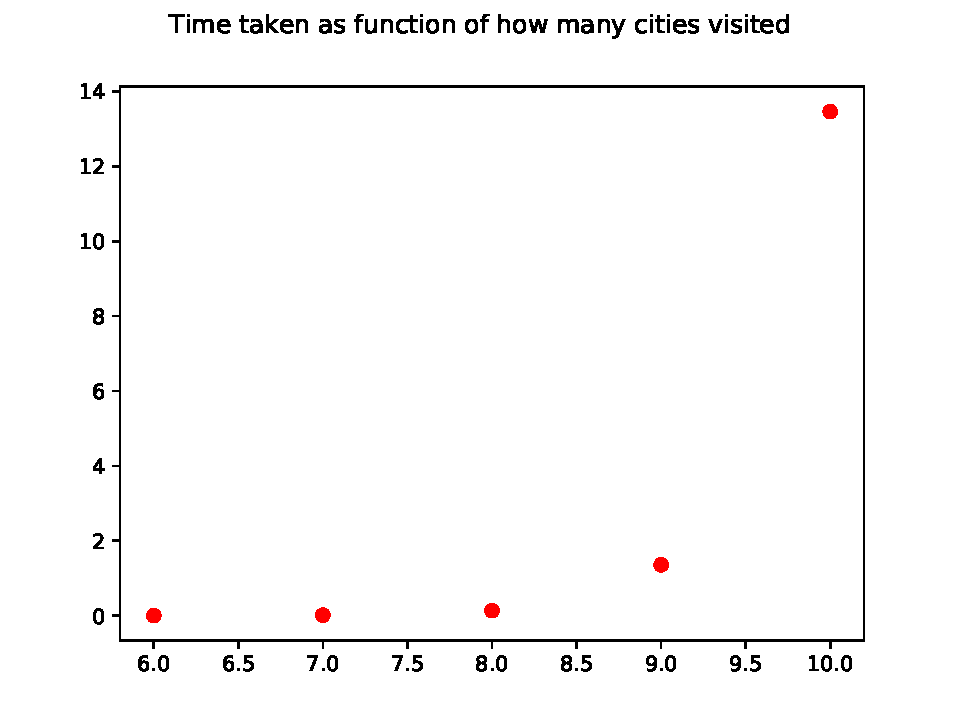
\includegraphics[scale=0.8]{"../Exhaustive.pdf}
\caption{Time spent for the TSP algorithm}
\end{center}
\end{figure}

It can be seen that the time spent by the algorithm searching the TSP for \textit{n} cities is roughly the time spent on calculating with \textit{n-1} cities multiplied by \textit{n}. The time spent by the algorithm to search TSP for 24 cities can be calculated with
\[
	t_{10} \frac{24!}{10!} \approx 14s \cdot \frac{24!}{10!} \approx 2.4 \cdot 10^{18}
\]


\section{Hill Climbing}

Start the program with
\begin{lstlisting}[language=bash]
	$ python3 hill_climber.py european_cities.csv 
\end{lstlisting}
Compare with exhaustive for 10 cities, run algorithm 20 times, report best worst mean and standard deviation for 10 runs and 24 runs
\section{Genetic algorithm}
Report parameters used, report best worst mean and deviation of 20 runs with three different values for population size, plot of average fitness of best individual of each run
\section{Hybrid algorithm}
Use hill climber on each individual as part of the evaluation, report min max mean deviation and average fitness with both Lamarckian and Baldwinian learning models, Compare result with GA

\end{document}
